% status: 100
% chapter: Amazon

\title{Amazon AWS EC2}


\author{Sushant Athaley}
\affiliation{%
  \institution{Indiana University} }
\email{sathaley@iu.edu}

% The default list of authors is too long for headers}
\renewcommand{\shortauthors}{G. v. Laszewski}


\begin{abstract}

AWS EC2 is a cloud infrastructure offering from Amazon which provides
compute resource virtualization. We explore AWS EC2 technology to
understand how we can use compute resource in a cloud environment.

\end{abstract}

\keywords{hid-sp18-402, i516, Amazon, AWS, EC2, Cloud, VM}

\maketitle

\section{Introduction}

The emergence of cloud computing is changing the paradigm the way we
are working with IT resources. It is helping to virtualize various IT
resources and eliminating the need for on-premise infrastructure. EC2
is one such service which provides computation capability in the
cloud. We evaluate EC2 as technology to understand various feature
provided by the service and how it is getting used to solving
practical problems.

We get started with the section \emph{Cloud} which explains the
concept of Cloud and various cloud offerings. Section \emph{EC2}
provides an introduction to the EC2 technology. Then we explore
technology in detail through subsections \emph{E-Elastic} which
captures elasticity in EC2, \emph{Instances and AMIs} captures various
software and hardware options, \emph{Integrated} captures integration
information, \emph{Security} explains security features
provided, \emph{Storage} explores various storage options
and \emph{Pricing} captures pricing information to use EC2.
Section \emph{Working with EC2} explores various ways to work with
EC2. Section \emph{Real Life Use Cases} talks about real life EC2
usage examples. Section \emph{Conclusion} concludes the study.

\section{Cloud}

In order to understand EC2, it's imminent that we understand the
concept of Cloud as EC2 is nothing but a cloud offering and it is
backed up by various feature and benefits provided by the Cloud
technology. Cloud's one of the easiest interpretation is something
which can be done over the internet instead of using our own CPU or
storage~\cite{hid-sp18-402-www-infoworld}. It is a new concept where
instead of using the traditional way of setting up IT infrastructure
to get the IT work done and then maintain it, commercially developed
infrastructure is used remotely over the internet. It virtualizes and
centralizes the whole IT infrastructure required by the
enterprise. Cloud is often backed up by massive infrastructure which
provides an ability to quickly upscale and downscale the required
resources like compute, storage, network and can use ready to use
proven pre-built services. Customer perspective, cloud enables them to
get new capabilities on demand without bothering about analysis and
investment need to be made on procuring new software or hardware. It
cuts down on the time involved to create the infrastructure as this
resources are already pre-built and readily available for use through
the cloud and can be set up within minutes for the usage. Scaling up
or down of the resources automatically based on a demand is one of the
biggest advantage provided by cloud infrastructure. Instead of paying
for entire infrastructure at once, the cloud provides an option to pay
per use which might be the cheaper alternative and important
consideration for any business operation.

There are various cloud services available like Software as a Service
(SaaS), Infrastructure as a Service (IaaS), Platform as a Service
(PaaS) and Function as a Service
(FaaS)~\cite{hid-sp18-402-www-infoworld}. The topic of this study, EC2
is IaaS offering and provides compute capability in the Amazon AWS
environment.

\section{EC2}

EC2 is a commercial web service offering from Amazon. Amazon describes
Elastic Compute Cloud which is referred as EC2 is a web service which
provides compute capacity in the cloud along with security and re-size
features~\cite{hid-sp18-402-www-aws-ec2}. In general, we can think of
it as a virtual computer in the cloud which can be used similarly to a
physical computer. It can be used as a server, development instance,
personal computer, deployment environment, test environment, virtual
machine or many more ways depending on the need. An EC2 instance can
have an operating system from the variety of the ranges available like
Windows, Amazon Linux, CentOS, and Debain along with the option of
uploading your own operating
system~\cite{hid-sp18-402-www-aws-ec2-details}. An EC2 instance can be
loaded with a custom application environment and can be configured to
work with various AWS or other services. As this is a cloud offering
it comes with various benefits offered by the cloud technology as well
as the massive infrastructure provided by Amazon.

\subsection{E-Elastic}
E in EC2 stands for Elastic which provides capability to increase and
decrease capacity on demand but also maintains the desired capacity
required. It can be used to commission hundred to thousands of
instances simultaneously based on the
requirement~\cite{hid-sp18-402-www-aws-ec2}. This is an important
feature of EC2 as it helps control computing power needed based on the
demand and provides optimized performance.  Amazon EC2 Auto
Scaling~\cite{hid-sp18-402-www-aws-ec2autoscaling} feature enables
configuration of various rules which are used to maintain or scale the
instances.
\subsubsection{Fleet Management}
EC2 Auto Scaling offers \emph{Fleet Management} which periodically
monitors the health of running instances and replaces faulty instances
by terminating that instance and replacing it with the new instance
automatically. The number of instances can be configured during fleet
configuration and auto-scaling will ensure that those number of
instances are up and running all the time without any downtime or
impact to the users.
\subsubsection{Dynamic Scaling}
Dynamic Scaling enables to increase or decrease the capacity based on
a parameter like CPU utilization where new instance will be added or
removed after certain CPU utilization is reached. This mechanism helps
in load balancing and provides the optimized performance to the
users. It can result in cost saving as resources are optimized as per
the rules configured.

Figure~\ref{f:ec2-auto-scaling} shows EC2 Auto Scaling.
\begin{figure}[!ht]
  \centering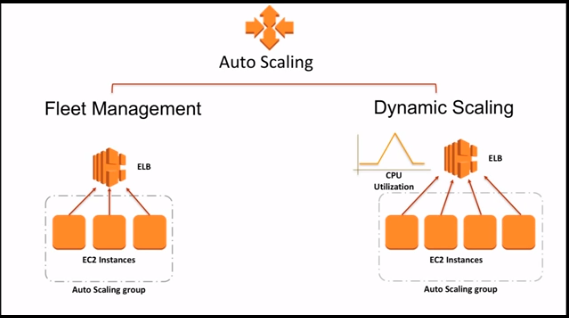
\includegraphics[width=\columnwidth]
	{images/ec2AutoScaling.PNG} \caption{EC2
  Auto
  Scaling~\cite{hid-sp18-402-www-aws-ec2autoscaling}}\label{f:ec2-auto-scaling}
\end{figure}

\subsection{Instances and AMIs}
EC2 provides flexibility to use the variety of instances which is
based on CPU, memory, storage, and the networking capability. Each
instance type provides various combinations of those parameters to
choose appropriate computing capability required as per the use
case. This helps in optimizing resources and cost based on the
workload. These instances are divided into various categories as
General Purpose, Compute Optimized, Memory Optimized, Storage
Optimized and Accelerated Computing. To get an idea of instance type
provided by EC2 we are taking lowest and highest configuration
available. In general category the smallest instance
type \emph{t2.nano} would have configuration as 1 vCPU, 0.5GB memory,
low networking performance with Intel Xeon processor 3.3GHz whereas
the higher end instance type \emph{m4.16xlarge} would have
configuration as 64vCPU, 256GB memory, 25GB networking speed with
Intel Xeon E5-2686v4 processor
2.3GHz~\cite{hid-sp18-402-www-aws-ec2instance}. There are many more
such configurations available which can be readily picked up and
deployed as EC2 instance without waiting for hardware procurement.

Amazon Machine Image (AMI)~\cite{hid-sp18-402-www-aws-ec2instance} is
a pre-configured image of the required operating system, software,
servers, databases, and applications. AMI is used to launch an
instance which in turn uses selected AMI to run on the instance. There
are predefined AMIs which can be readily used but also custom AMI can
be created as per the need.

Figure~\ref{f:ec2-ami-instance} shows EC2 AMI and Instance
relationship.
\begin{figure}[!ht]
  \centering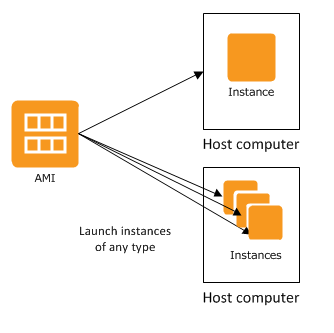
\includegraphics[width=\columnwidth]
{images/ec2AMI.PNG} \caption{EC2
  Instance and
  AMI~\cite{hid-sp18-402-www-aws-ec2instance}}
\label{f:ec2-ami-instance}
\end{figure}

\subsection{Integrated}
EC2 is backed by various services offered by AWS and can be integrated
with those services. AWS S3, AWS RDC, AWS VPC are some of the services
which can be used in conjunction with EC2 to develop different
applications~\cite{hid-sp18-402-www-aws-ec2}.
Figure~\ref{f:ec2-integration} shows sample EC2 integration with S3,
RDS and EBS.
\begin{figure}[!ht]
  \centering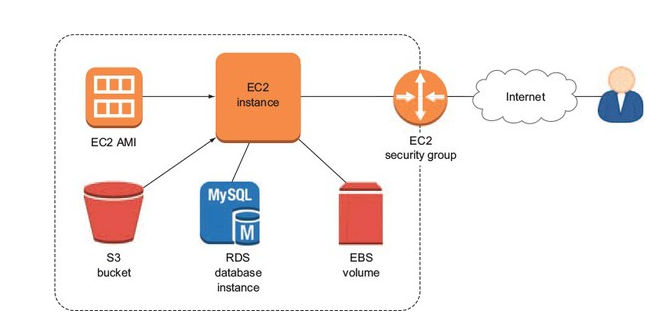
\includegraphics[width=\columnwidth]
{images/ec2Integration.PNG} \caption{EC2
  Integration~\cite{hid-sp18-402-www-medium-aws}}
\label{f:ec2-integration}
\end{figure}

\subsection{Security}
Security in EC2 is provided on multiple levels like operating system
authentication on the instance, guest OS, firewall and signed API
calls. Host operating system itself has security and access mechanism
built in which can restrict unauthorized access. Guest OS itself is a
less privileged access system which doesn't allow critical
operations. EC2 provides firewall solution which is used to restrict
traffic on certain ports as well as for certain protocols and IP
addresses. Inbound traffic requires explicitly port opening and
specific group policy can be applied to access those ports. Remote
access through API calls can only be made if secret access key is
created and established using
EC2~\cite{hid-sp18-402-www-aws-ec2Security}.

\subsection{Storage}
Data storage and processing are essential capabilities for many of the
compute operations. EC2 provides various options for the data storage
and those options have their own characteristics in terms of
performance and
durability~\cite{hid-sp18-402-www-aws-ec2Storage}. Figure~\ref{f:ec2-storage}
shows relationship between various storage types provided by EC2.
\begin{figure}[!ht]
  \centering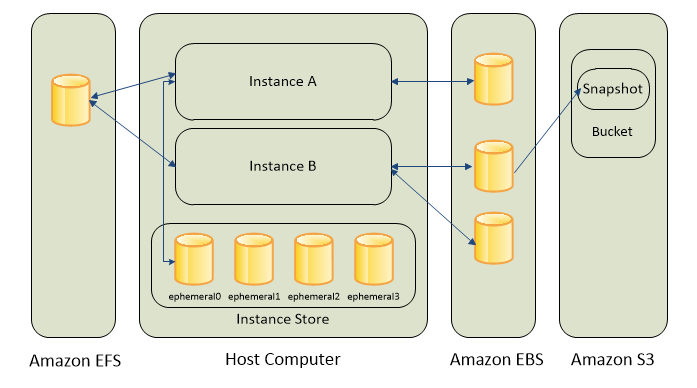
\includegraphics[width=\columnwidth]
{images/ec2Storage.PNG} \caption{EC2
  Storage
  Types~\cite{hid-sp18-402-www-aws-ec2Storage}}
\label{f:ec2-storage}
\end{figure}

\subsubsection{Amazon EC2 Instance Store} 
Instance store~\cite{hid-sp18-402-www-aws-ec2Storage} is a temporary
storage attached as a physical disk to the host computer. This can be
used as a temporary storage like a buffer, cache, scratch data as it
is lost in case of instance stopped, terminated or disk drive is
failed.
\subsubsection{Amazon Elastic Block Store (EBS)} 
EBS provides durable block-level storage to the EC2 instance. This
storage is independent of instance life cycle and can be used as
primary storage type for the EC2. This is a persistent storage and can
be attached to multiple instances. EBS can be used as a database
storage. It also provides encryption
capabilities~\cite{hid-sp18-402-www-aws-ec2Storage}.
\subsubsection{Amazon Elastic File System (EFS)} 
EFS provides file system storage to the EC2
instance~\cite{hid-sp18-402-www-aws-ec2Storage}. This is a persistent
storage which can be used or shared between multiple instances.
\subsubsection{Amazon Simple Storage Service (S3)} 
S3 is persistent and instance independent data store which is suitable
for data movement and storage in large volume. This storage can be
accessed through EC2 as well as from outside over the
web~\cite{hid-sp18-402-www-aws-ec2Storage}.

\subsection{Pricing}
EC2 is a commercial offering from Amazon and it offers various pay
models which can be used as per the need. It also offers free option
to try if the micro instance is used.
\subsubsection{On-Demand} 
This option allows to pay on per hour or per the second basis based on
the instance usage~\cite{hid-sp18-402-www-aws-ec2Pricing}.
\subsubsection{Spot Instances} 
Spot instances are the spare instances and offered at steep discounts
based on the biding. Spot instance can be interrupted at any point if
the EC2 instance needs its capacity
back~\cite{hid-sp18-402-www-aws-ec2Pricing}.
\subsubsection{Reserved Instances} 
Reserved instance offers discounted rates compared to on-demand rates
based on the commitment provided by the customer. Reserved instance
provides capacity reservation to launch instance as required which
ensures the instance
availability~\cite{hid-sp18-402-www-aws-ec2Pricing}.
\subsubsection{Dedicated Hosts} 
The dedicated host provides a dedicated physical EC2 instance for the
usage. This can be useful if any compliance or regulatory requirement
needs to be met by the
business~\cite{hid-sp18-402-www-aws-ec2Pricing}.

\section{Working with EC2}
There are 3 different ways which can be used to interact with EC2. To
use EC2, first we need to create an AWS account and then complete
related setup like creation of IAM (Identity and Access Management)
user to access, creation of key pair for secure access, creation of
virtual private cloud (VPC) to lunch instance in user-defined virtual
network and creation of security group which acts as a
firewall~\cite{hid-sp18-402-www-aws-ec2-setup}.

\subsection{Management Console}
Management Console~\cite{hid-sp18-402-www-aws-ec2-gettingStarted} is a
web-based user interface to access various AWS resources. Log in to
the management console and select EC2 from the list to start working
with EC2. This interface provides the capability to configure, launch,
connect and terminate an instance.

\subsection{Command Line Tool}
AWS CLI (Command Line Interface)~\cite{hid-sp18-402-www-aws-ec2-cli}
is the command line interface provided by Amazon to interact with
various AWS web services. This open source tool is built on top of the
AWS SDK for Python. These commands can be used from Linux shells,
windows command line and remotely through a remote terminal like
PuTTY. To use AWS CLI, it needs to be installed using \emph{pip} on
Linux, macOS, or Unix environment and on Windows using MSI
installer. AWS CLI need to be configured by setting key and region
before it can be used to work with an EC2 instance.
Figure~\ref{c:cli-launch} shows sample CLI command to launch an
instance.
\begin{figure}[htb]
\begin{verbatim}
aws ec2 run-instances --image-id ami-6e1a0117 --security-group-ids
sg-b018ced5 --count 1 --instance-type t2.micro --key-name devenv-key
--query 'Instances[0].InstanceId'
\end{verbatim}
\caption{Launch Instance~\cite{hid-sp18-402-www-aws-ec2-cli}}
\label{c:cli-launch}
\end{figure}

\subsection{SDKs}
AWS services can be accessed through various platforms or programming
languages which enables a developer to work with AWS in their
preferred programming language. These platforms or language-specific
libraries are called as SDK. Currently, SDKs are available
for \emph{Android, Browser, iOS, Java, Microsoft~.Net, Node.js, PHP, Python,
Ruby, Go,} and \emph{C++}~\cite{hid-sp18-402-www-aws-ec2-sdk}.

\section{Real Life Use Cases}
Any technology can be understood better by understanding real-life
examples of how it is being used practically to solve any problem or
use case. In this section, we explore some examples of EC2 usage from
real life.

\subsubsection{Netflix}
Netflix is one of the good examples of cloud platform usage as well as
AWS usage. Netflix completed their migration to AWS cloud in 2016
which lasted over the period of 7
years~\cite{hid-sp18-402-www-media-netflix}. Netflix uses numerous
services provided by AWS out of which EC2 is used as computing service
which hosts Netflix's various customer facing as well as internal
applications. It also hosts Cassandra Database, Elasticsearch, and
EVCache. It uses EC2 Linux cloud with thousands of virtual server
instances along with the autoscale feature to support over 50M
subscribers~\cite{hid-sp18-402-www-brendangregg}.

\subsubsection{Airbnb}
Airbnb is a community marketplace for finding vacation rentals and
having more than 9 million users. They require massive storage along
with the efficient rental booking application to support growing
request load. Airbnb uses AWS EC2, elastic load balancing, EMR, S3,
Cloudwatch, and Amazon RDS. It uses about 200 EC2 instances for
application hosting, Memcache and search
servers~\cite{hid-sp18-402-www-aws-ec2-airbnb}.

\subsubsection{Novartis}
Novartis is a pharmaceutical company involved in drug discovery and
innovation. They wanted to run the complex algorithm to screen 10
million compounds against common cancer target which would require
huge computing capability along with the storage. They used AWS EC2,
S3, and EBS to build a program which ran on multiple instances
simultaneously to complete the matching. They used 10,600 EC2 spot
instances to run the
algorithm~\cite{hid-sp18-402-www-aws-ec2-novartis}.

\subsubsection{Lamborghini}
Lamborghini is an automotive company which was facing issue with the
outdated infrastructure and non-scalable environment they were using
to host their website. They decided to migrate their website to AWS
and used AWS ELB, EC2, RDS, S3, CloudFront, and Cloudwatch in their
architecture~\cite{hid-sp18-402-www-aws-ec2-lamborghini}. It is not
clear from the available documentation that how they are using EC2 in
their design but our guess is, EC2 is getting used as a web-server
host for the web application.

\section{Conclusion}
EC2 is a commercial web service provided by Amazon. This is an
Infrastructure as a Service (IaaS) cloud offering which provides
compute capability. EC2 provides features like elastic auto-scaling,
flexible hardware and software configurations, integrations with other
AWS web services, access security using secure key and firewall
configurations, data storage options and flexible price options. It
also provides an interactive web interface to work with the EC2
instances at the same time SDKs in various programming languages to
work with EC2 in a programmatic way. One of the biggest advantages of
EC2 is the infrastructure provided by Amazon which helps to create
thousands of instances in very less time which is helpful for solving
big data or any other problems which require a lot of computing
capability. The robust features and flexibility offered by EC2 make it
as one of the preferred virtual compute resource.

\begin{acks}

  The author would like to thank Dr.~Gregor~von~Laszewski for his
  support and suggestions to write this paper.

\end{acks}

\bibliographystyle{ACM-Reference-Format}
\bibliography{report} 
